\thispagestyle{pagenumberonly}

\subsection{Eigenschaften von Mengen}

\begin{notation}[Konkrete Beschreibung von Mengen]
    Eine Menge ist informell formuliert eine Ansammlung von Objekten.
    Um diese Objekte konkret anzugeben, schreiben wir $M = \set{1, 2, 3}$.\\
    Eine andere Möglichkeit, eine Menge anzugeben ist über die Eigenschaften der Elemente.
    Wir schreiben: $M=\set{x|~H(x)}$. Das bedeutet, dass ein Element $x$ genau dann ein Element der Menge ist, wenn $H(x)$ gilt.
    Wir schreiben $x\in M \equivalent H(x)$.
\end{notation}

\begin{beispiel}[Mengendeklaration über Aussagenform]
    \begin{align*}
        H(x) &\definedas (x^2-3x+2 = 0)\\
        \impl \set{x|~H(x)} &= \set{1,2}
    \end{align*}
\end{beispiel}

\begin{definition}[Eigenschaften von Mengen]
    Allgemein gilt für Mengen:
    \theoremescape
    \begin{enumerate}
        \item 2 Mengen sind gleich, wenn sie die selben Elemente enthalten.
        \item Die leere Menge ($\emptyset$) ist die einzige Menge, die keine Elemente enthält.
        \item Wenn für jedes $x\in A$ auch $x\in B$ folgt, dann ist $A$ eine Teilmenge von $B$. ($A\subseteq B$)
        \item Ist $A\subseteq B$ und $A\neq B$, dann nennen wir $A$ eine echte Teilmenge von $B$. ($A\subsetneq B$)
        \item $A$ und $B$ sind disjunkt, falls aus $x\in A$ folgt, dass $x\not\in B$.
    \end{enumerate}
\end{definition}

\begin{bemerkung}
    Allgemein gilt für zwei Mengen $A$ und $B$, dass $A\subseteq B \land B\subseteq A \equivalent A = B$.\footnote{Diese Äquivalenz wird insbesondere in Beweisen häufig eingesetzt, indem durch das Zeigen, dass zwei Mengen gegenseitige Teilmenge sind, deren Gleichheit gezeigt wird.}
\end{bemerkung}

\subsection{Operationen mit Mengen}

\begin{definition}[Mengenoperationen]
    Seien $A, B$ Mengen. Dann gilt:
    \begin{align*}
        A\cap B &\definedas \set{x|~x\in A \land x\in B}\tag{Schnitt}\\
        A\cup B &\definedas \set{x|~x\in A \lor x\in B}\tag{Vereinigung}\\
        A\exclude B &\definedas \set{x|~x\in A \land x\notin B}\tag{Differenz}\\[10pt]
        \text{Wenn } A\subseteq M&\colon A^{C} = A^{C}_{M} \definedas M\exclude A\tag{Komplement}
    \end{align*}
    Allgemein gilt: $A$ und $B$ disjunkt $\equivalent A\cap B = \emptyset$
\end{definition}

\begin{visualisierung}[Darstellung von Mengen als Venn-Diagramm]
    Die Operationen auf zwei Mengen $A$ und $B$ lassen sich mittels eines Venn-Diagramms veranschaulichen:
    \begin{figure}[H]
        \centering
        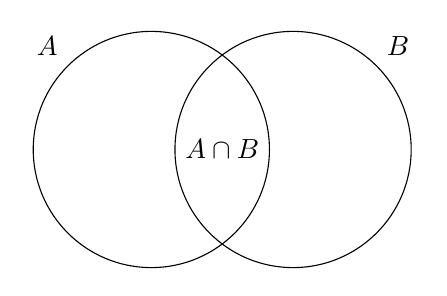
\begin{tikzpicture}
            \node [draw,
            circle,
            minimum size =3cm,
            label={135:$A$}] (A) at (0,0){};

            \node [draw,
            circle,
            minimum size =3cm,
            label={45:$B$}] (B) at (1.8,0){};
            \node at (0.9,0) {$A\cap B$};
        \end{tikzpicture}
        \caption{Schnittmenge zweier Mengen als Venn-Diagramm}
    \end{figure}
\end{visualisierung}

%%%%%%%%%%%%%%%%%%%%%%%%
% 31. Oktober 2023
%%%%%%%%%%%%%%%%%%%%%%%%

\begin{lemma}[Kommutativität des Schnitts]
    \marginnote{[31. Okt]}
    $A\cap B = B \cap A$
    \begin{proof}
        \begin{align*}
            A\cap B &= \set{x|~x\in A \land x \in B}\\
            &= \set{x|~x\in B \land x \in A}\\
            &= B\cap A\qedhere
        \end{align*}
    \end{proof}
\end{lemma}

\begin{lemma}[Distributivität]
    $A\cup (B \cap C) = (A\cup B) \cap (A\cup C)$
    \begin{proof}
        \begin{align*}
            x\in A \cup \pair{B \cap C} &\equivalent x\in A \lor x\in B \cap C\\
            &\equivalent x\in A \lor \pair{x\in B \land x \in B}\\
            &\equivalent \pair{x\in A \lor x\in B}\land\pair{x\in A \lor x\in C}\\
            &\equivalent x\in A \cup B\land x \in A \cup C\\
            &\equivalent x\in \pair{A \cup B}\cap\pair{A\cup C}\qedhere
        \end{align*}
    \end{proof}
\end{lemma}

\begin{definition}[Familie von Mengen]
    Sei $J$ eine Indexmenge mit $J\neq \emptyset$. Die Mengenfamilie ist gegeben durch Mengen $A_{j}$ für jedes $j\in J$. Wir schreiben $\set{A_j}_{j\in J}$
\end{definition}

\begin{definition}[Schnitt und Vereinigung über mehrere Mengen]
    Für eine Mengenfamilie $\set{A_j}j\in J$ gilt:
    \begin{align*}
        \bigcap_{j\in J} A_j &\definedas \set{x|~\forall j\in J: x\in A_j}\\[10pt]
        \bigcup_{j\in J} A_j &\definedas \set{x|~\exists j\in J: x\in A_j}
    \end{align*}
\end{definition}

\subsection{Quantoren}

\begin{definition}[Quantoren]
    Wir definieren drei unterschiedliche Quantoren:
    \theoremescape
    \begin{enumerate}[label=(\roman*)]
        \item $\forall$: \anf{Für alle}
        \item $\exists$: \anf{Es existiert ein}
        \item $\exists!$: \anf{Es existiert genau ein}
    \end{enumerate}
    \vspace{0.2cm}
    Es seien $A,B$ Mengen und $H(x,y)$ eine Aussageform mit $x\in A$ und $y \in B$. Dann gilt:
    \begin{align*}
        \forall x \in A~\exists y \in B\colon H(x,y) \equivalent \text{Für alle $x\in A$ existiert ein $y \in B$, so dass $H(x,y)$ wahr ist}
    \end{align*}
\end{definition}

\begin{folgerung}[Negation von Quantoren]
    Es seien $A,B$ Mengen und $H(x,y)$ Aussageform mit $x\in A$ und $y \in B$. Dann gilt:
    \begin{align*}
        \neg\pair{\forall x \in A\colon H(x)} &\equivalent \exists x\in A\colon \neg H(x)\\
        \neg\pair{\exists x \in A\colon H(x)} &\equivalent \forall x\in A\colon \neg H(x)\\
        \neg \pair{\forall x \in A~\exists y\in B\colon H(x,y)}&\equivalent\exists x \in A\colon \neg\pair{\exists y\in B\colon H(x,y)}\\
        &\equivalent \exists x\in A~\forall y \in B\colon \neg H(x,y)\\
    \end{align*}
\end{folgerung}

\begin{definition}[Potenzmenge und Mengensystem]
    Sei $A$ eine Menge, so heißt $\mathcal{P}(A) \definedas \set{N|~N \subseteq A}$ Potenzmenge von $A$. Eine Teilmenge $A\subseteq \mathcal{P}(A)$ heißt Mengensystem über $A$.
\end{definition}

\begin{bemerkung}[Russels Paradoxon]
    Russel definiert: $R\definedas\set{M|~M \text{ ist Menge und $M \notin M$}}$\\
    Falls $R$ eine Menge, dann kann man fragen, ob $R\in R$ oder nicht.\\
    1. Fall: $R\notin R\impl R\in R$\qquad (Widerspruch)\\
    2. Fall: $R\in R\impl R \notin R$\qquad (Widerspruch)\\
    Lösung: $R$ ist keine Menge, sondern eine Klasse.
\end{bemerkung}

\vfill

\subsection{Kartesisches Produkt und Relationen}

\begin{definition}[Tupel]
    Seien $A$ und $B$ Mengen. Für $x\in A$ und $y\in B$ ist $(a,b) \definedas \set{a, \set{a,b}}$ das geordnete Paar oder Tupel bestehend aus $a$ und $b$.\\[10pt]
    Zwei Tupel $(a_1, b_1)$ und $(a_2, b_2)$ mit $a_1, a_2\in A, b_1, b_2\in B$ sind genau dann gleich, wenn ihr jeweils erstes und zweites Element gleich ist:
    \begin{align*}
    (a_1, b_1)
        = (a_2, b_2) \equivalent a_1 = a_2 \land b_1 = b_2
    \end{align*}
\end{definition}

\begin{definition}[Kartesisches Produkt]
    Somit ist $A \times B \definedas \set{\pair{a,b}|~a\in A \land b \in B}$ wieder eine Menge, genannt das Kartesische Produkt von $A$ und $B$.
\end{definition}

\begin{beispiel}
    \begin{align*}
        M &\definedas \set{1,2,3}\\
        N &\definedas \set{3,4}\\
        M\times N &= \set{(1,3), (1,4), (2,3), (2,4), (3,3), (3,4)}
    \end{align*}
\end{beispiel}


\begin{definition}[Relation]
    Seien $A, B$ Mengen. Eine Relation $R=\pair{A, B, G}$ besteht aus einer Menge $A$, einer Menge $B$ und einer Menge $G\subseteq A\times B$.\\
    $G$ ist der Graph von $R$, auch geschrieben als $G_R$.
    Ist $\pair{a,b}\in G$ so sagt man \anf{$a$ ist $R$-verwandt zu $b$}. Wir schreiben $aRb$ (Infix-Schreibweise).\\
    $A$ ist die Definitionsmenge von $R$ und $B$ ist die Zielmenge von $R$.\\[10pt]
    Seien $R_1 = \pair{A_1, B_1, G_1}$ und $R_2 = \pair{A_2, B_2, G_2}$ Relationen. Dann gilt:
    \begin{align*}
        R_1 = R_2 \equivalent A_1 = A_2 \land B_1 = B_2 \land G_1 = G_2
    \end{align*}
    Wir können eine Umkehrrelation $R^{-1}$ wie folgt definieren:
    \begin{align*}
        R^{-1} &\definedas \pair{B,A,G_{R^{-1}}}\\
        G_{R^{-1}} &\definedas \set{\pair{b,a} |~\pair{a,b} \in G_R}
    \end{align*}
\end{definition}

\begin{beispiel}[Kleiner-Relation]
    Es sei $A = \set{1,2,3,4}$. Wir definieren die Kleiner-Relation $R=\set{A, A, G_{<}}.$\\
    Dann gilt: $a_1 < a_2 \equivalent \pair{a_1, a_2} \in G_{<}$ und somit $G_{<} = \set{(1,2), (1,3), (1,4), (2,3), (2,4), (3,4)}$
\end{beispiel}

\vfill
\newpage

\begin{definition}[Äquivalenzrelation]
    Sei $R=\pair{A, A, G}$ eine Relation. Dann definieren wir unterschiedliche Eigenschaften, die die Relation haben kann:
    \begin{enumerate}[label=(\roman*)]
        \item $R$ ist reflexiv:\quad $\forall a\in A\colon aRa\quad\pair{\forall a \in A\colon (a,a) \in G}$
        \item $R$ ist symmetrisch:\quad $\forall a_1, a_2\in A\colon a_{1}Ra_2\equivalent a_{2}Ra_1$
        \item $R$ ist transitiv:\quad $\forall a_1, a_2, a_3 \in A\colon a_{1}Ra_{2} \land a_{2}Ra_{3} \impl a_{1}Ra_{3}$
    \end{enumerate}
    Eine Äquivalenzrelation ist eine reflexive, symmetrische und transitive Relation auf $A$.\\
    Ist $R$ eine Äquivalenzrelation und $a_{1}Ra_{2}$ so nennt man $a_{1}$ äquivalent zu $a_{2}$ bezüglich $R$.
\end{definition}

\begin{notation}[Äquivalenzklassen]
    Sei $R$ Äquivalenzrelation auf $A$. Dann gilt:
    \begin{align*}
    [a]
        _{R} \definedas \set{b\in A|~aRb}
    \end{align*} ist die Äquivalenzklasse von $a$. Wir schreiben auch $a\sim_R b$ für $aRb$ oder $a = b$ modulo $R$.
\end{notation}

\begin{beobachtung}
    Allgemein gilt für Äquivalenzklassen damit:
    \theoremescape
    \begin{enumerate}[label=(\roman*)]
        \item $\forall a\in A\colon [a]_R \neq \emptyset$
        \item $aRa \impl a\in [a]_R$
        \item $a_1, a_2\in [a]_R \impl a_1 \sim_R a, a_2 \sim_R a \annot{\impl}{sym.} a_1 \sim_R a, a \sim_R a_2 \annot{\impl}{trans.} a_1\sim_R a_2$
    \end{enumerate}
\end{beobachtung}

\begin{lemma}
    Sei $R$ Äquivalenzrelation auf $A$. Für $a_1,a_2\in A$ ist entweder $[a_1]_R = [a_2]_R$ oder $[a_1]_R \cap [a_2]_R = \emptyset$.
    \begin{proof}
        Da $[a_1]_R$, $[a_2]_R \neq \emptyset$ reicht es zu zeigen, dass: $[a_1]_R \cap [a_2]_R \neq \emptyset \impl [a_1]_R = [a_2]_R$.
        \begin{align*}
            \text{Sei }b\in [a_1]_R\cap [a_2]_R\text{ und }c\in [a_1]_R\\
            \impl b\sim_R a_1 \land c\sim_R a_1 \annot{\impl}{trans.} c\sim_R b\\
            \intertext{Da  $b\sim_R a_2$ muss nach der Transitivität gelten:}
            c\sim_R a_2 \impl [a_1]_R \subseteq [a_2]_R
        \end{align*}
        Symmetrisch lässt sich argumentieren, dass $[a_2]_R \subseteq [a_1]_R$.
    \end{proof}
\end{lemma}

\begin{korollar}
    Es sei $R$ eine Äquivalenzrelation auf $A\neq \emptyset$. Dann sind $a_1,a_2\in A$ entweder äquivalent oder sie gehören zu disjunkten Äquivalenzklassen.
\end{korollar}

\begin{definition}[Zerlegung einer Menge]
    Sei $A\neq \emptyset$ eine Menge. Dann ist eine Zerlegung $F = \set{A_j}_{j\in J}, A_j\subseteq A$ mit folgenden Eigenschaften definiert:
    \begin{enumerate}
        \item $\forall j\in J\colon A_j\neq \emptyset$
        \item Für $j_1, j_2\in J, j_1\neq j_2\colon A_{j1} \cap A_{j2} = \emptyset$
        \item $\bigcup_{j\in J}A_j = A$
    \end{enumerate}
\end{definition}

\begin{notation}[Quotient]
    Es sei $R$ Äquivalenzrelation auf $A$.
    \begin{align*}
        F\definedas\set{[a]_R|~a\in A}
    \end{align*}
    ist eine Zerlegung von $A$ (bezüglich der Äquivalenzrelation $R$). Wir schreiben $F = A/R$.
    $A/R$ ist der \anf{Quotient} von $A$ bezüglich $R$
\end{notation}

\begin{beispiel}[Restklassendefinition über Äquivalenzrelationen]
    Es sei $A = \naturalnumbers_{0} = \set{0,1,2,3,4,\dots}$ und $p\in \mathbb{N}$. $m,n\in\mathbb{N}_0$ seien genau dann äquivalent, wenn $m=n+k\cdot p$ für ein $k\in\mathbb{Z}$:
    \begin{align*}
        R_{p} = \set{\pair{m,n}\in \mathbb{N}_0 \times \mathbb{N}_0 |~\exists k\in \mathbb{Z}\text{ mit } m=n+k\cdot p}
    \end{align*}
    So definieren wir die Restklassen von $\mathbb{N}_0$ bezüglich Division mit $p$.
    \begin{align*}
        m\in [j]_{R} \equivalent m=n+k\cdot p\text{ für ein }k\in\mathbb{Z}
    \end{align*}
\end{beispiel}

%%%%%%%%%%%%%%%%%%%%%%%%
% 2. November 2023
%%%%%%%%%%%%%%%%%%%%%%%%

\subsection{Funktionen}

\begin{bemerkung}[Moralische Definition einer Funktion]
    \marginnote{[2. Nov]}
    Gegeben Mengen $A, B$, eine Relation $f$ von $A$ nach $B$. $f$ ist eine Funktion, wenn es jedem Element in $A$ genau ein Element in $B$ zuordnet.
\end{bemerkung}

\begin{notation}[Pfeilnotation]
    Wir schreiben $f: A \fromto B,~a\mapsto f\pair{a}$.
\end{notation}
\begin{folgerung}
    Zu $a\in A$ gibt es $f\pair{a}\in B \leadsto$ Tupel($a, f\pair{a}$) $\in A\times B \impl \set{\pair{a, f(a)}: a\in A} \subseteq A\times B$.
\end{folgerung}

\begin{definition}[Funktion]
    Eine Relation $R = (A, B, G_R)$ heißt Funktion (oder Abbildung), wenn
    \begin{align*}
        \forall a\in A~\exists! b\in B\colon (a,b)\in G_f.
    \end{align*}
    Wir setzen dann $f(a)\definedas b$.
\end{definition}

\begin{beispiel}[Mögliche Funktionen]
    \theoremescape
    \begin{alignat*}{2}
        f\colon &\mathbb{Z} \rightarrow \realnumbers,\quad && n\mapsto 3n^2+7\\
        g\colon &\mathbb{Z} \rightarrow \mathbb{Z},\quad && n\mapsto 3n^2+7\\
        h\colon &\linterv{0, \infinity} \rightarrow \realnumbers,\quad && x\mapsto x^2+3x+4\\
        j\colon &\realnumbers \rightarrow \realnumbers,\quad && x\mapsto x^2+3x+4\\
    \end{alignat*}
\end{beispiel}
\begin{bemerkung}
    $f$ und $g$ haben zwar die gleiche Funktionsvorschrift, sind aber dennoch unterschiedliche Funktionen, da diese wie Relationen auch über Definitionsmenge und Zielmenge definiert sind.
\end{bemerkung}

\begin{notation}[Bild und Urbild]
    Sei $f: A\rightarrow B$ eine Funktion.
    Dann gilt
    \begin{alignat*}{2}
        & M \subseteq A:~ & f\pair{M} &\definedas \set{b\in B|~\exists x\in M\colon b=f\pair{x}}\tag{Bild von $M$ unter $f$}\\
        & N \subseteq B:~ & f^{-1}\pair{N} &\definedas \set{a\in A|~f(a)\in N}\tag{Urbild von $N$ unter $f$}
    \end{alignat*}
    Außerdem ist das gesamte Bild von $f$ definiert als
    \begin{align*}
        Bild(f) \definedas f(A)
    \end{align*}
\end{notation}
\begin{definition}[Einschränkungen von Funktionen]
    Sei $f\colon~A \rightarrow B$ eine Funktion und $M \subseteq A$.
    Dann ist die Einschränkung (oder Restriktion) von $f$ auf $M$ definiert als
    \begin{align*}
        f|_{M}\colon&~M \rightarrow B,\quad x \mapsto f\pair{x}
    \end{align*}
\end{definition}
\begin{definition}[Besondere Eigenschaften von Funktionen]
    Es sei $f\colon A\fromto B$ eine Funktion.
    \theoremescape
    \begin{enumerate}[label=(\roman*)]
        \item $f$ ist injektiv, falls $\forall a_1, a_2 \in A\colon f\pair{a_1} = f\pair{a_2} \impl a_1 = a_2$.
        \item $f$ ist surjektiv, falls $Bild\pair{f} = B$.
        \item $f$ ist bijektiv, falls es injektiv und surjektiv ist. In diesem Fall existiert eine Inverse\\ $f^{-1}: B\fromto A, b\mapsto a$ mit $f(a)=b$.
    \end{enumerate}
\end{definition}

\subsection{Geordnete Mengen}

\begin{definition}[Ordnungsrelation und teilweise geordnete Menge]
    Es sei $A$ eine Menge und $R$ eine Relation auf $A$. $R$ heißt Ordnungsrelation (geschrieben \anf{$\prec$}), falls
    \begin{enumerate}[label=(\roman*)]
        \item $\forall a\in A\colon a \prec a$ (Reflexivität)
        \item $\forall a_1, a_2, a_3\in A\colon a_1\prec a_2 \land a_2 \prec a_3 \impl a_1 \prec a_3$ (Transitivität)
        \item $\forall a_1, a_2\in A\colon a_1\prec a_2 \land a_2 \prec a_1 \impl a_1 = a_2$ (Antisymmetrie)
    \end{enumerate}
    $\pair{A, \prec}$ heißt \textbf{teilweise} geordnete Menge. Nicht alle Paare $a_1$, $a_2$ müssen vergleichbar sein.
\end{definition}

\begin{notation}
    Wir schreiben $a_1\prec a_2$ als $a_{1}Ra_{2}$ oder $\pair{a_1, a_2}\in G_R$.
\end{notation}
\begin{definition}[Kette]
    $T\subseteq A$ heißt Kette (oder geordnete Menge), falls
    \begin{align*}
        a_1, a_2\in T \impl a_1\prec a_2 \lor a_2 \prec a_1
    \end{align*}
\end{definition}

\begin{beispiel}[Ordnungsrelation]
    Ordnungsrelation auf $\mathcal{P}(A)$:
    \begin{align*}
        M, N \subseteq A \quad M \prec N, \text{ falls } M\subseteq N
    \end{align*}
    \noindent Ordnungsrelation auf $\naturalnumbers$:
    \begin{align*}
    (\naturalnumbers, \prec)
        : n\prec m, \text{ falls $n$ teilt $m$}
    \end{align*}
    $2$ und $3$ sind dabei nicht vergleichbar, aber $2$ und $4$ sind vergleichbar.
\end{beispiel}

\newpage